%
% $RCSfile: cybernetics_oriented_interpreter.tex,v $
%
% Copyright (C) 2002-2008. Christian Heller.
%
% Permission is granted to copy, distribute and/or modify this document
% under the terms of the GNU Free Documentation License, Version 1.1 or
% any later version published by the Free Software Foundation; with no
% Invariant Sections, with no Front-Cover Texts and with no Back-Cover
% Texts. A copy of the license is included in the section entitled
% "GNU Free Documentation License".
%
% http://www.cybop.net
% - Cybernetics Oriented Programming -
%
% http://www.resmedicinae.org
% - Information in Medicine -
%
% Version: $Revision: 1.1 $ $Date: 2008-08-19 20:41:06 $ $Author: christian $
% Authors: Christian Heller <christian.heller@tuxtax.de>
%

\chapter{Cybernetics Oriented Interpreter}
\label{cybernetics_oriented_interpreter_heading}
\index{Cybernetics Oriented Interpreter}
\index{CYBOI}

\begin{flushright}
    \textsl{
        Two Things are needed to do our Work:\\
        tireless Endurance and the Willingness to throw something,\\
        that has cost much Time and Effort, away again.
    }\\
    \textsc{Albert Einstein}
\end{flushright}

The previous chapter described how the CYBOP concepts introduced in part
\ref{contribution_heading} of this work can be implemented in a formal language
carrying the abbreviated name CYBOL. The now still missing piece is a program
able to dynamically handle static CYBOL sources, as mentioned in chapter
\ref{statics_and_dynamics_heading}. This chapter therefore describes the
\emph{Cybernetics Oriented Interpreter} (CYBOI) \cite{cybop} which can do just
that.

%
% $RCSfile$
%
% Copyright (c) 2005-2006. Christian Heller. All rights reserved.
%
% Permission is granted to copy, distribute and/or modify this document
% under the terms of the GNU Free Documentation License, Version 1.1 or
% any later version published by the Free Software Foundation; with no
% Invariant Sections, with no Front-Cover Texts and with no Back-Cover
% Texts. A copy of the license is included in the section entitled
% "GNU Free Documentation License".
%
% http://www.cybop.net
% - Cybernetics Oriented Programming -
%
% http://www.resmedicinae.org
% - Information in Medicine -
%
% Version: $Revision$ $Date$ $Author$
% Authors: Christian Heller <christian.heller@tuxtax.de>
%

\subsubsection{Architecture}
\label{architecture_heading}

To what concerns its inner architecture, there are two basic structures
underlying CYBOI:

\begin{enumerate}
    \item \emph{Knowledge Container:} An array-based structure usable for
        storing static knowledge in form of primitive- and compound models, and
        capable of representing a map, collection, list and tree
    \item \emph{Signal Checker:} A loop-based structure usable for dynamically
        reading signals from a queue, and capable of processing them after
        their priority, in a special handler
\end{enumerate}

\begin{figure}[ht]
    \begin{center}
        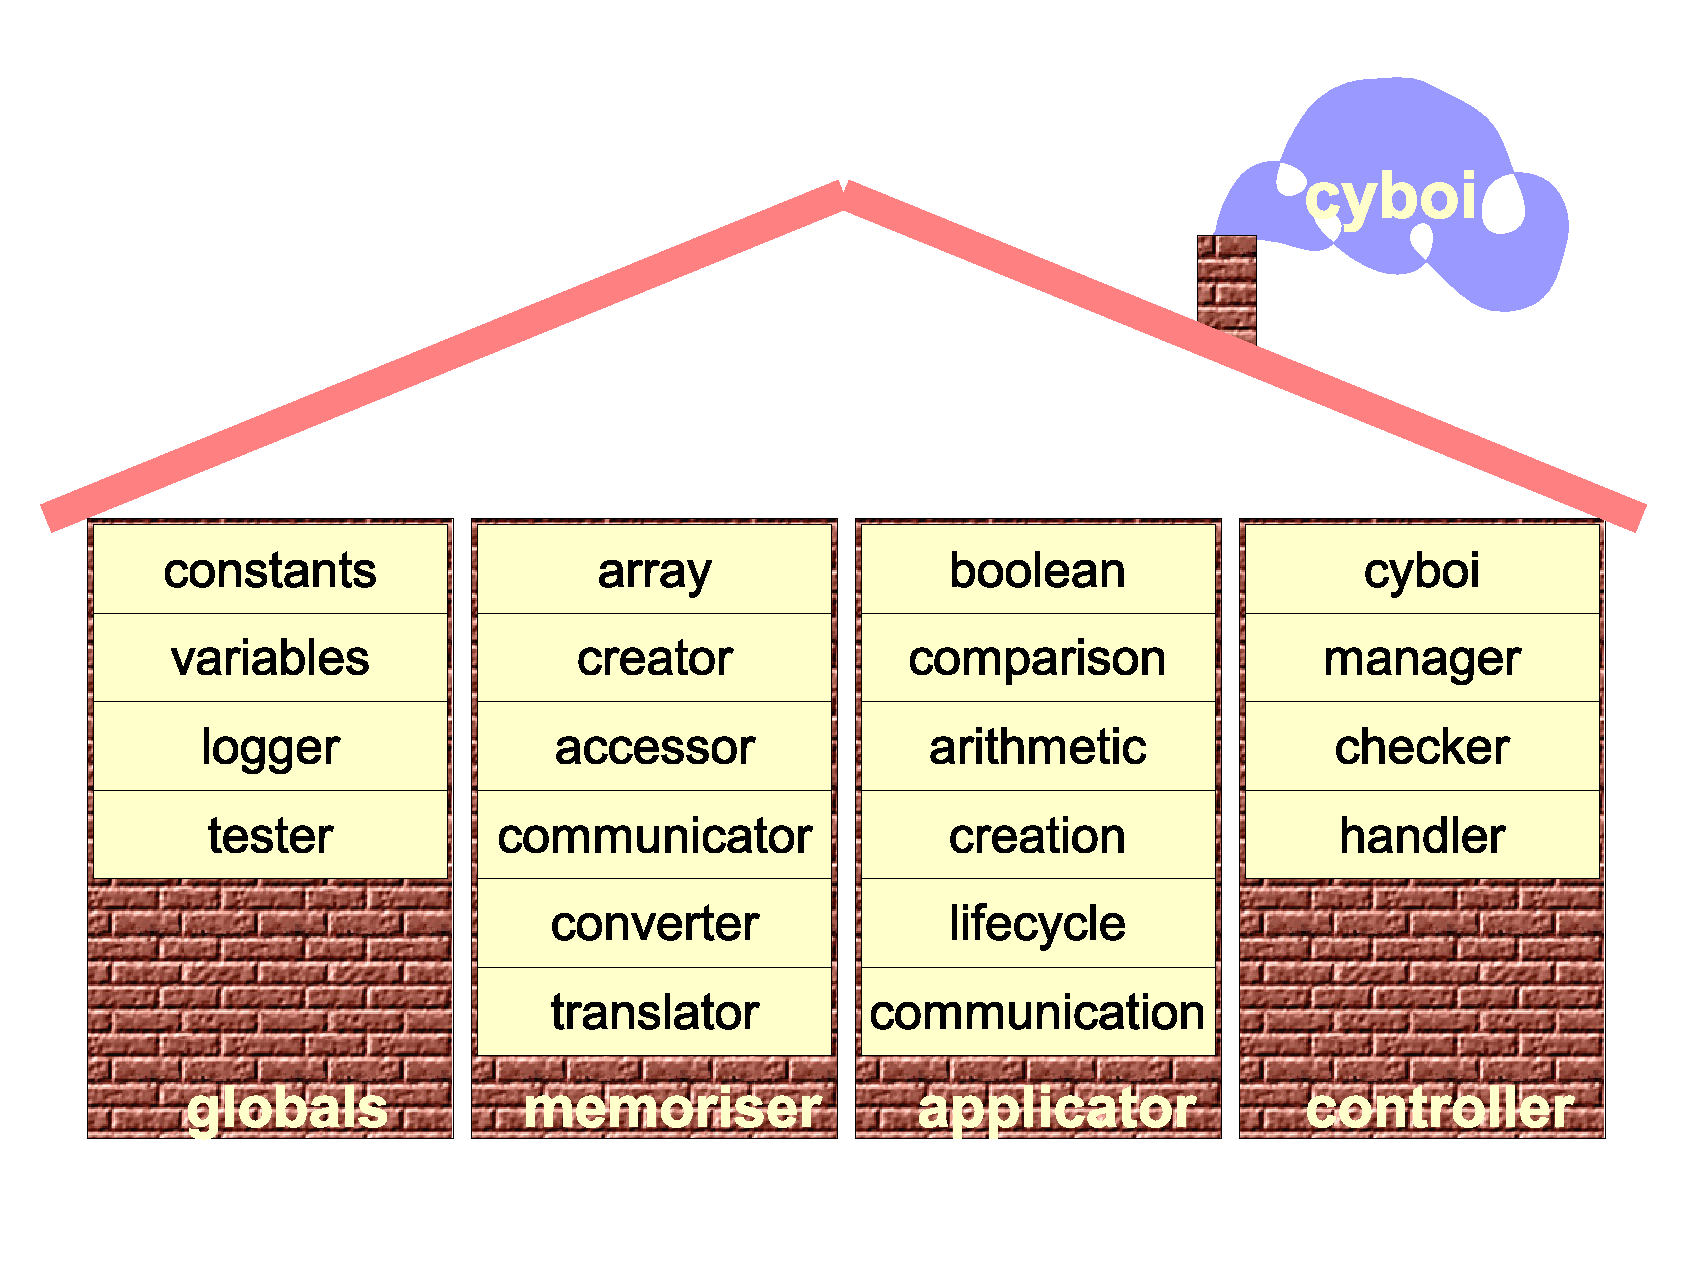
\includegraphics[scale=0.2]{vector/architecture.eps}
        \caption{CYBOI Architecture}
        \label{architecture_figure}
    \end{center}
\end{figure}

All modules, into which CYBOI is subdivided, are built around these two core
structures. Not unlike John von Neumann's model of a computing machine
\cite{selflinux}, which distinguishes \emph{Memory}, \emph{Control Unit},
\emph{Algorithmic Logic Unit} (ALU) and \emph{Input/ Output} (i/o), CYBOI's
modules are grouped into four architectural parts, as illustrated in figure
\ref{architecture_figure}. These have the following functionality:

\begin{itemize}
    \item \emph{Memoriser:} data creation, -destruction and -access (after
        Neumann, it contains not only data, but also the operations that are
        applied to them)
    \item \emph{Controller:} lifecycle management, signal handling, i/o filters
    \item \emph{Applicator:} operation application (comparison, logic,
        arithmetic and more)
    \item \emph{Globals:} basic constants and variables, as well as a logger
\end{itemize}

The i/o data handling is not separated out here (as opposed to von Neumann's
model); it is managed by the controller modules. The i/o data themselves,
representing states, are stored in memory.

%
% $RCSfile: functionality_in_detail.tex,v $
%
% Copyright (C) 2002-2008. Christian Heller.
%
% Permission is granted to copy, distribute and/or modify this document
% under the terms of the GNU Free Documentation License, Version 1.1 or
% any later version published by the Free Software Foundation; with no
% Invariant Sections, with no Front-Cover Texts and with no Back-Cover
% Texts. A copy of the license is included in the section entitled
% "GNU Free Documentation License".
%
% http://www.cybop.net
% - Cybernetics Oriented Programming -
%
% http://www.resmedicinae.org
% - Information in Medicine -
%
% Version: $Revision: 1.1 $ $Date: 2008-08-19 20:41:06 $ $Author: christian $
% Authors: Christian Heller <christian.heller@tuxtax.de>
%

\section{Functionality in Detail}
\label{functionality_in_detail_heading}
\index{CYBOI Functionality}
\index{CYBOI Part Dependencies}
\index{CYBOI Control Flow}

CYBOI's architecture is based on three main parts, as introduced by figure
\ref{architecture_figure} before: \emph{Controller}, \emph{Applicator} and
\emph{Memoriser}. (The \emph{Globals} package is neglectable for the following
explanations, since it contains static constants and variables that are
\emph{omnipresent}.) They appear again in figure \ref{dependencies_figure}
which shows the \emph{Dependencies} between them. Additionally, the
\emph{Controller} modules and their \emph{Control Flow} is illustrated.
Starting from the \emph{cyboi} module, the following subsections will
demonstrate how CYBOI functions internally, along the flow of control touching
the modules: \emph{manager}, \emph{checker} and \emph{handler}. After that, the
execution of operations in the \emph{Applicator} as well as the creation and
transition of data in the \emph{Memoriser} are described.

\begin{figure}[ht]
    \begin{center}
        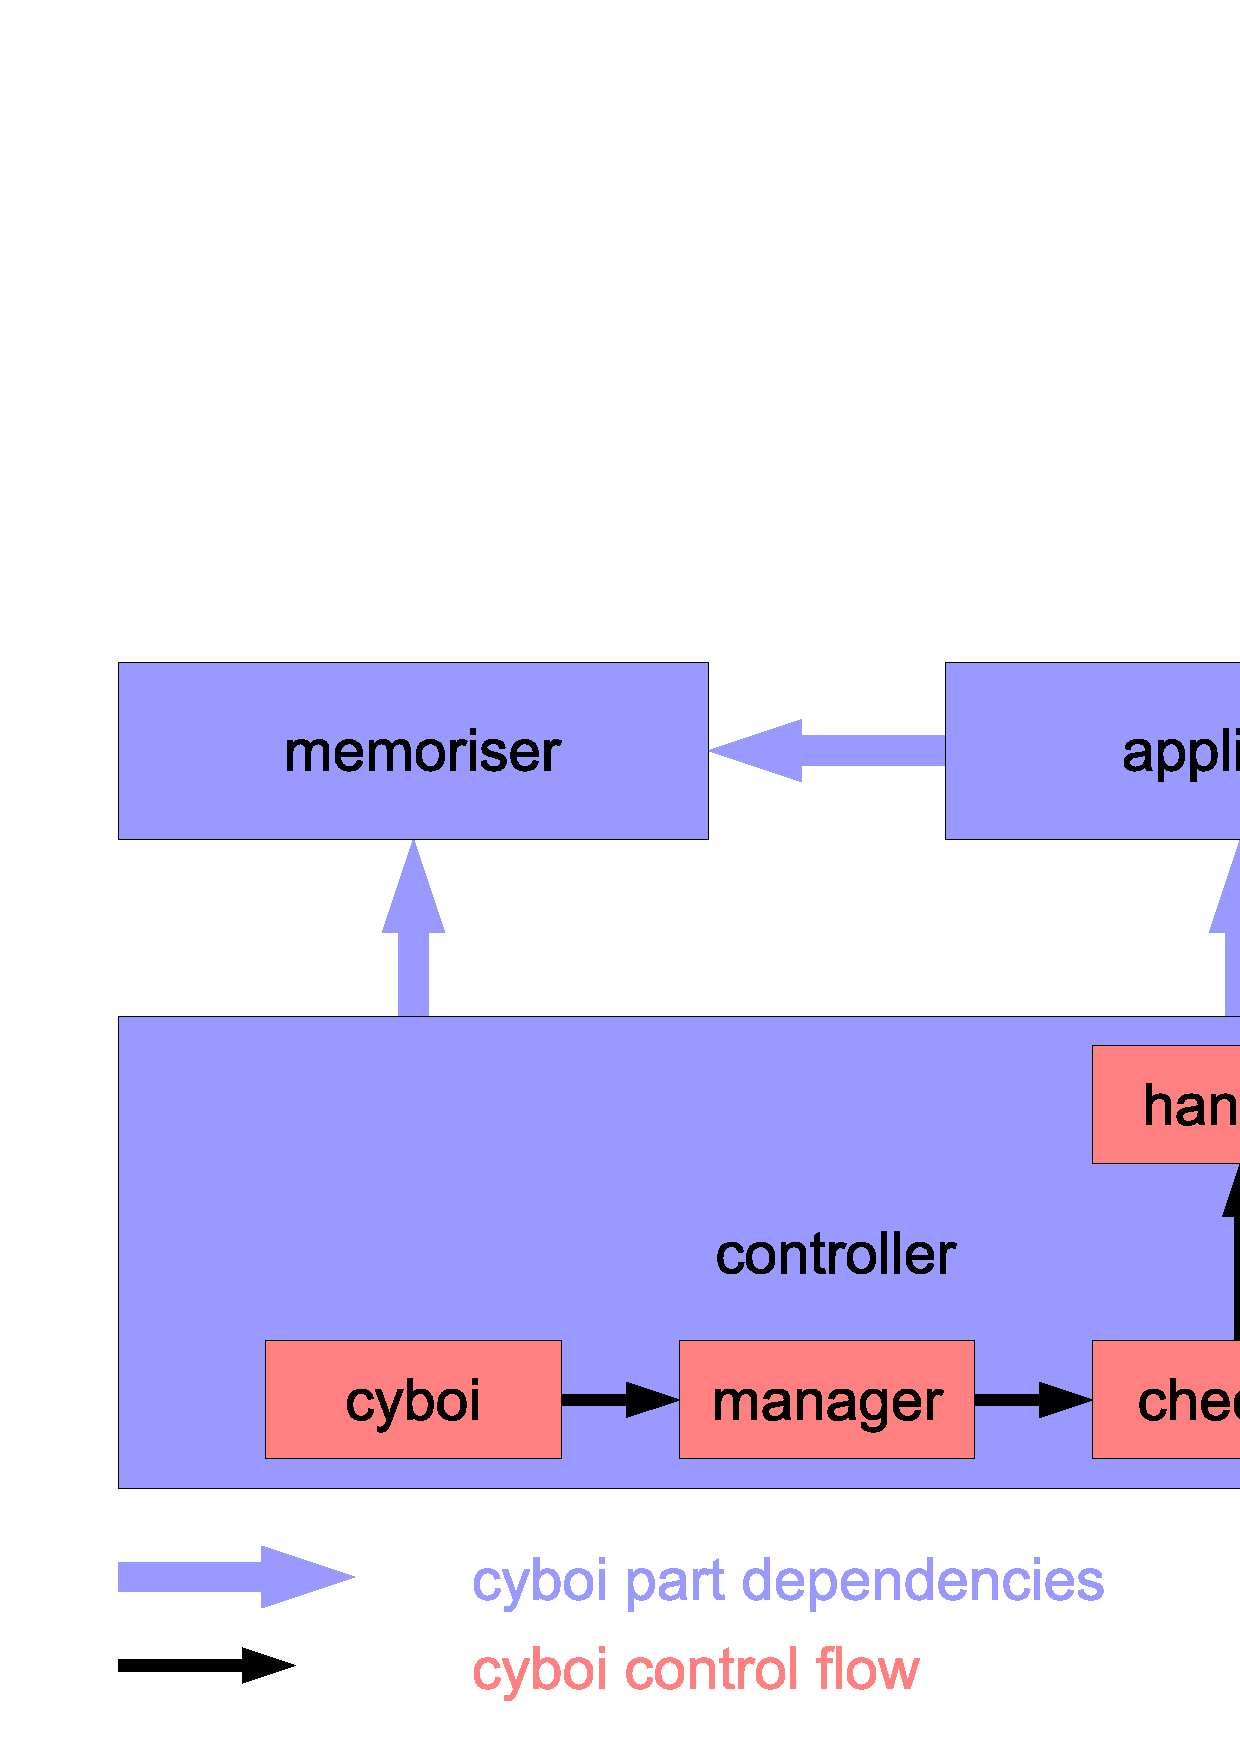
\includegraphics[scale=0.3,angle=-90]{graphic/dependencies.pdf}
        \caption{CYBOI Part Dependencies and Control Flow}
        \label{dependencies_figure}
    \end{center}
\end{figure}

%
% $RCSfile: process_launching.tex,v $
%
% Copyright (C) 2002-2008. Christian Heller.
%
% Permission is granted to copy, distribute and/or modify this document
% under the terms of the GNU Free Documentation License, Version 1.1 or
% any later version published by the Free Software Foundation; with no
% Invariant Sections, with no Front-Cover Texts and with no Back-Cover
% Texts. A copy of the license is included in the section entitled
% "GNU Free Documentation License".
%
% http://www.cybop.net
% - Cybernetics Oriented Programming -
%
% http://www.resmedicinae.org
% - Information in Medicine -
%
% Version: $Revision: 1.1 $ $Date: 2008-08-19 20:41:08 $ $Author: christian $
% Authors: Christian Heller <christian.heller@tuxtax.de>
%

\subsection{Process Launching}
\label{process_launching_heading}
\index{CYBOI Process Launching}
\index{CYBOI main Procedure}

As every other C-, C++- or Java program, CYBOI has a \emph{main} procedure
(\emph{cyboi} module) serving as entry point for its process to run. It
triggers the system lifecycle (in the meaning of startup and shutdown of a
system process). After having initialised global variables and having read the
command line parameter, the rest of the system is started up by the
\emph{manage} procedure (\emph{manager} module).

%
% $RCSfile: lifecycle_management.tex,v $
%
% Copyright (C) 2002-2008. Christian Heller.
%
% Permission is granted to copy, distribute and/or modify this document
% under the terms of the GNU Free Documentation License, Version 1.1 or
% any later version published by the Free Software Foundation; with no
% Invariant Sections, with no Front-Cover Texts and with no Back-Cover
% Texts. A copy of the license is included in the section entitled
% "GNU Free Documentation License".
%
% http://www.cybop.net
% - Cybernetics Oriented Programming -
%
% http://www.resmedicinae.org
% - Information in Medicine -
%
% Version: $Revision: 1.1 $ $Date: 2008-08-19 20:41:07 $ $Author: christian $
% Authors: Christian Heller <christian.heller@tuxtax.de>
%

\subsection{Lifecycle Management}
\label{lifecycle_management_heading}
\index{CYBOI Lifecycle Management}

To the startup routine belong the creation of the three containers: knowledge
memory, signal memory and internals memory, and the creation of a startup model
which is placed as first signal into the signal memory. Additional meta
information given are the signal's model, its kind of abstraction and priority.

Typical synonyms for \emph{Signal} are \emph{Event} or \emph{Action} -- and
even an \emph{Operating System} (OS) \emph{Interrupt} is some form of signal,
only on a lower system level, closer to hardware. In CYBOI, a signal is simply
a reference to a logic model, which may be either a composed algorithm, or a
primitive operation.

With the startup signal being placed in the signal memory, the system enters
the \emph{check} procedure (\emph{checker} module). On shutdown, the system
runs through similar procedures in opposite direction, only that then startup
signal, memories and global variables are destroyed.

%
% $RCSfile: signal_checking.tex,v $
%
% Copyright (C) 2002-2008. Christian Heller.
%
% Permission is granted to copy, distribute and/or modify this document
% under the terms of the GNU Free Documentation License, Version 1.1 or
% any later version published by the Free Software Foundation; with no
% Invariant Sections, with no Front-Cover Texts and with no Back-Cover
% Texts. A copy of the license is included in the section entitled
% "GNU Free Documentation License".
%
% http://www.cybop.net
% - Cybernetics Oriented Programming -
%
% http://www.resmedicinae.org
% - Information in Medicine -
%
% Version: $Revision: 1.1 $ $Date: 2008-08-19 20:41:08 $ $Author: christian $
% Authors: Christian Heller <christian.heller@tuxtax.de>
%

\subsection{Signal Checking}
\label{signal_checking_heading}
\index{CYBOI Signal Checking}

The \emph{check} procedure consists of an endless loop continuously checking
for signals residing in signal memory. It provides the dynamics and -- so to
say -- keeps the system \emph{alive}. Of all queued signals, the one with
highest priority is retrieved first and forwarded to the \emph{handle}
procedure (\emph{handler} module).

This principle can be observed not only in operating-, but many other kinds of
systems. \emph{Servers} run an endless loop waiting for (network) \emph{Client}
requests. Applications often use signalling mechanisms provided by a framework,
that handles keyboard press- or mouse click signals stemming from a
\emph{Graphical User Interface} (GUI). However, as opposed to the event
handling of such frameworks which relies on bidirectional dependencies since
child components have to register as listener at their parent, a top-level
signal checker loop forwards all events in a unidirectional manner to
interested system parts. It is worth noting that signals may also be produced
internally, as follow-ups, by other signals.

After having been processed, the signal gets removed from the signal memory.
Once an \emph{exit} signal occurs, the shutdown flag is set, so that the signal
checking loop can be left -- and the system be shutdown.

%
% $RCSfile: signal_handling.tex,v $
%
% Copyright (C) 2002-2008. Christian Heller.
%
% Permission is granted to copy, distribute and/or modify this document
% under the terms of the GNU Free Documentation License, Version 1.1 or
% any later version published by the Free Software Foundation; with no
% Invariant Sections, with no Front-Cover Texts and with no Back-Cover
% Texts. A copy of the license is included in the section entitled
% "GNU Free Documentation License".
%
% http://www.cybop.net
% - Cybernetics Oriented Programming -
%
% http://www.resmedicinae.org
% - Information in Medicine -
%
% Version: $Revision: 1.1 $ $Date: 2008-08-19 20:41:08 $ $Author: christian $
% Authors: Christian Heller <christian.heller@tuxtax.de>
%

\subsection{Signal Handling}
\label{signal_handling_heading}
\index{CYBOI Signal Handling}
\index{Central Processing Unit}
\index{CPU}

Depending on the signal model's kind of abstraction, two different signal
handling procedures may be called: \emph{handle\_compound} or
\emph{handle\_operation} (both in the \emph{handler} module). While the former
breaks down composed signals (algorithms) into basic operations, the latter
executes primitive signals (operations) directly, in form of low-level
instructions, which may go down to direct calls of the instruction set of the
\emph{Central Processing Unit} (CPU).

Actual knowledge model changes, in other words the application of well-defined
\emph{Logic-} to \emph{State} models, is done by primitive operations only.

%
% $RCSfile: operation_execution.tex,v $
%
% Copyright (C) 2002-2008. Christian Heller.
%
% Permission is granted to copy, distribute and/or modify this document
% under the terms of the GNU Free Documentation License, Version 1.1 or
% any later version published by the Free Software Foundation; with no
% Invariant Sections, with no Front-Cover Texts and with no Back-Cover
% Texts. A copy of the license is included in the section entitled
% "GNU Free Documentation License".
%
% http://www.cybop.net
% - Cybernetics Oriented Programming -
%
% http://www.resmedicinae.org
% - Information in Medicine -
%
% Version: $Revision: 1.1 $ $Date: 2008-08-19 20:41:08 $ $Author: christian $
% Authors: Christian Heller <christian.heller@tuxtax.de>
%

\subsection{Operation Execution}
\label{operation_execution_heading}
\index{CYBOI Operation Execution}

Each low-level operation has its own module, belonging to the \emph{Applicator}
part of CYBOI. An addition operation is executed in the \emph{add} module, a
comparison operation in the \emph{compare} module, a creation operation in the
\emph{create} module, and so forth. Operations exist for several purposes, some
of which are listed, together with an example operation, following:

\begin{itemize}
    \item[-] program flow (\emph{loop})
    \item[-] boolean logic (\emph{and})
    \item[-] comparison (\emph{equals})
    \item[-] arithmetics (\emph{add})
    \item[-] service control (\emph{startup})
    \item[-] memory management (\emph{create})
\end{itemize}

%
% $RCSfile: model_transition.tex,v $
%
% Copyright (C) 2002-2008. Christian Heller.
%
% Permission is granted to copy, distribute and/or modify this document
% under the terms of the GNU Free Documentation License, Version 1.1 or
% any later version published by the Free Software Foundation; with no
% Invariant Sections, with no Front-Cover Texts and with no Back-Cover
% Texts. A copy of the license is included in the section entitled
% "GNU Free Documentation License".
%
% http://www.cybop.net
% - Cybernetics Oriented Programming -
%
% http://www.resmedicinae.org
% - Information in Medicine -
%
% Version: $Revision: 1.1 $ $Date: 2008-08-19 20:41:07 $ $Author: christian $
% Authors: Christian Heller <christian.heller@tuxtax.de>
%

\subsection{Model Transition}
\label{model_transition_heading}
\index{CYBOI Model Transition}
\index{Knowledge Template}
\index{Knowledge Model}
\index{Information Processing Model}
\index{CYBOI as Universal Data Converter}

The creation of transient knowledge models (to be kept in memory, at runtime)
from persistent knowledge templates (given in form of CYBOL sources) is not a
trivial thing. It is a mechanism consisting of a cascade of model transitions,
comparable to the \emph{Information Processing Model} of cognitive psychology
(section \ref{information_processing_model_heading}). One may imagine this as a
state changing its appearance, while \emph{wandering} through the system. The
same mechanism is applied when handling communication data (figure
\ref{transition_figure}). Because CYBOI's architecture is easily extensible
with various modules, such as \emph{import/ export} (i/e) filters for different
kinds of communication, it may act as universal data converter. All
corresponding modules belong to the \emph{Memoriser} part of CYBOI.

\begin{figure}[ht]
    \begin{center}
        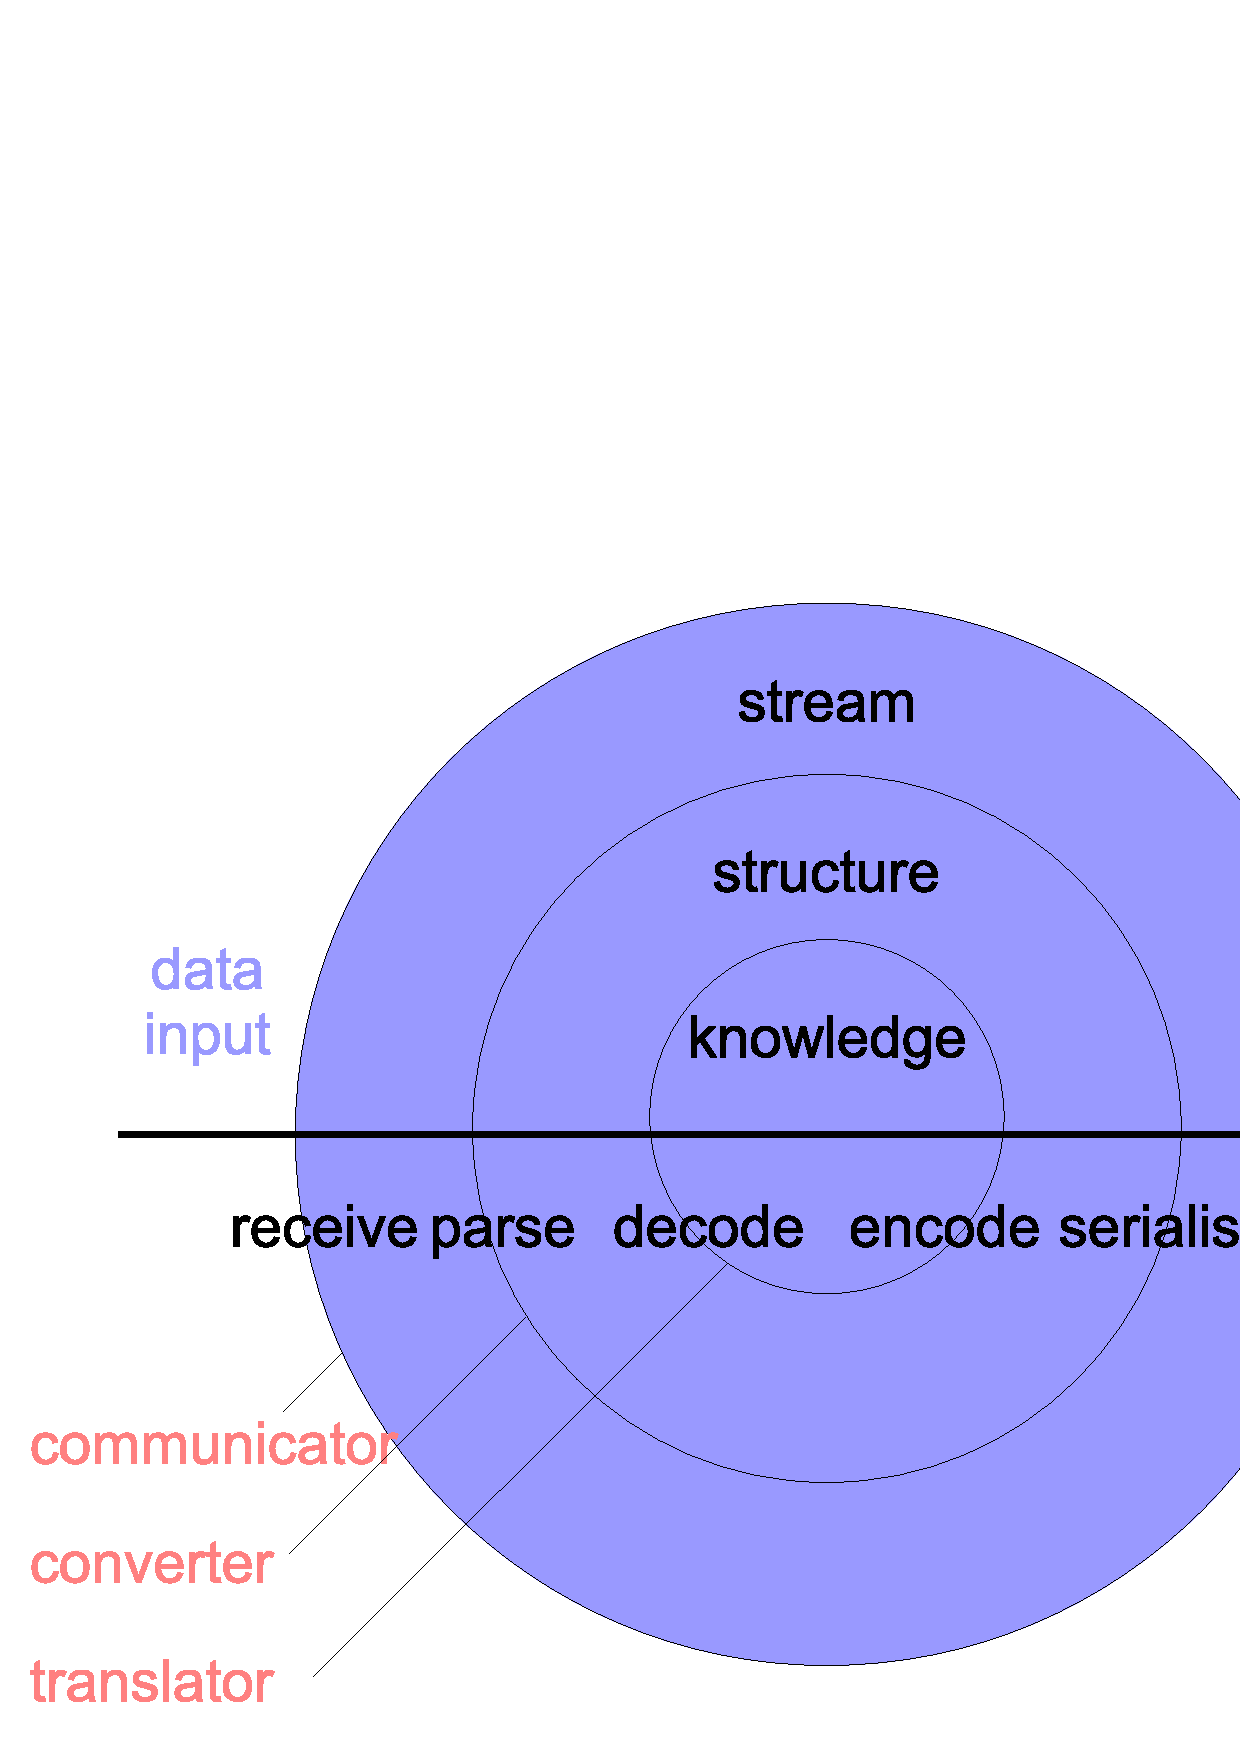
\includegraphics[scale=0.3,angle=-90]{graphic/transition.pdf}
        \caption{Input-to-Output Model Transition}
        \label{transition_figure}
    \end{center}
\end{figure}

As opposed to the knowledge acquirement in \emph{Artificial Neural Networks}
(ANN),
%(section \ref{artificial_neural_network_heading}),
the knowledge in CYBOP
systems is not learned, but \emph{injected} by reading from external knowledge
sources, which can be manipulated in a flexible manner any time. The difference
to standard applications is that these hard-wire their knowledge within the
system.

A data input (i/p), after having been processed by a \emph{receive} procedure
(\emph{communicator} modules), results in a stream -- a data array in memory. A
\emph{parse} procedure (\emph{converter} modules), depending on the kind of
abstraction of the data, then builds a structure out of this simple array. The
structure, finally, passes a \emph{decode} procedure (\emph{translator}
modules) which creates a knowledge model.

Whenever an application running within CYBOI wants to send data, may it be to
another system or for making them persistent on a local \emph{Hard Disk Drive}
(HDD), translator, converter and communicator have to be crossed in the
opposite direction. Because a running application system is a tree of knowledge
models allocating space in memory, parts of that tree can be \emph{serialised}
easily. It has to be mentioned, though, that slight changes of the XML format
are necessary to achieve this: The usual quotation marks used to delimit XML
attribute values have to be replaced with differing \emph{begin} and \emph{end}
characters. This feature is an open issue which the current version of CYBOI
does not provide yet.

%Isn't CYBOI model transition similar to termios Zeichenverarbeitung in Linux?
%siehe Grafik im Buch: Anwendungen entwickeln unter Linux, S. 249

%
% $RCSfile: data_creation.tex,v $
%
% Copyright (C) 2002-2008. Christian Heller.
%
% Permission is granted to copy, distribute and/or modify this document
% under the terms of the GNU Free Documentation License, Version 1.1 or
% any later version published by the Free Software Foundation; with no
% Invariant Sections, with no Front-Cover Texts and with no Back-Cover
% Texts. A copy of the license is included in the section entitled
% "GNU Free Documentation License".
%
% http://www.cybop.net
% - Cybernetics Oriented Programming -
%
% http://www.resmedicinae.org
% - Information in Medicine -
%
% Version: $Revision: 1.1 $ $Date: 2008-08-19 20:41:06 $ $Author: christian $
% Authors: Christian Heller <christian.heller@tuxtax.de>
%

\subsection{Data Creation}
\label{data_creation_heading}
\index{CYBOI Data Creation}
\index{CYBOI Data Encapsulation}
\index{Compound Structure as Multi Dimensional Container}
\index{Knowledge Memory consisting of Compound- and Primitive Models}

The functionality of CYBOI as system is built around the manipulation of states
in memory. The question how states, representing data, are stored is therefore
of great importance. Besides containers like the \emph{Internals Memory},
\emph{Knowledge Memory} and \emph{Signal Memory}, belonging to its
infrastructure, CYBOI uses special structures encapsulating primitive data. Not
only types like \emph{Character}, \emph{Integer}, \emph{Float} or \emph{String}
are wrapped this way, also \emph{Operations} are. Any compositions of these are
stored as \emph{Compound}.

Encapsulated primitives have the advantage of being forwardable as reference
(memory address pointer), instead of as copy. This ensures that redundant data
are avoided and states of manipulated primitives are not lost. \emph{Logic}
operations are stored in form of a string indicating their name. Necessary
references to input/ output (i/o) \emph{State} models need to be provided as
meta information, by the compound model surrounding the operation.

The \emph{Compound}, as most important CYBOI structure capable of representing
state- as well as logic knowledge, and capable of emulating a map, collection,
list and tree, deserves closer inspection. Essentially, it is a container able
to recursively reference instances of its own, thus spanning up a tree of parent
nodes (\emph{Whole} models) that may have child nodes (\emph{Part} models). In
fulfillment of the requirements of the knowledge schema introduced in section
\ref{knowledge_representation_heading}, a compound consists of a combination of
many arrays containing a part's:

\begin{itemize}
    \item[-] \emph{Name:} serving as unique \emph{Identifier} (ID)
    \item[-] \emph{Model:} the actual contents (may be a part node)
    \item[-] \emph{Abstraction:} the kind of abstraction (type) of the model
    \item[-] \emph{Details:} further meta information (properties, constraints)
\end{itemize}

One may call the \emph{Compound} a \emph{multi-dimensional} container but it is
probably easier described as large table with many columns, whereby the values
of one row describe exactly one part model, and thus belong together.

The previously mentioned \emph{Knowledge Memory} may be seen as huge tree
consisting of compound- as well as primitive models. Its root is always a
\emph{Compound} -- it, so to say, concentrates all knowledge in just one point,
the single concepts being branches of it.

The essential procedures for managing data in memory are \emph{create} and
\emph{destroy} (\emph{creator} modules). Three additional kinds of procedures
are provided for compound- and other container-like structures: \emph{set},
\emph{get} and \emph{remove} (\emph{accessor} modules). It should be noted at
this point that CYBOL applications have no direct access to these procedures,
so that \emph{wild} memory allocation is not possible. A knowledge model can
only be created using the corresponding CYBOL operation \emph{create\_part}.

%%
% $RCSfile: instance.tex,v $
%
% Copyright (C) 2002-2008. Christian Heller.
%
% Permission is granted to copy, distribute and/or modify this document
% under the terms of the GNU Free Documentation License, Version 1.1 or
% any later version published by the Free Software Foundation; with no
% Invariant Sections, with no Front-Cover Texts and with no Back-Cover
% Texts. A copy of the license is included in the section entitled
% "GNU Free Documentation License".
%
% http://www.cybop.net
% - Cybernetics Oriented Programming -
%
% http://www.resmedicinae.org
% - Information in Medicine -
%
% Version: $Revision: 1.1 $ $Date: 2008-08-19 20:41:07 $ $Author: christian $
% Authors: Christian Heller <christian.heller@tuxtax.de>
%

\subsection{Instance}
\label{instance_heading}

CYBOI Translator for model creation is NOT the same as a CYBOL translator model!

- while knowledge in a system exists as huge (transient) hierarchy,
it is defined in discrete (persistent) templates outside
- processing of source code (knowledge templates):
1 persistent model
2 transient received/read model
3 parsed model
4 decoded model

Application knowledge is kept in form of \emph{Templates} of which \emph{Instances}
can be created. Knowledge instances are \emph{Clones} (section \ref{clone_heading}).
Every knowledge instance can become a template itself.

While a knowledge instance is stored as one huge, serialisable tree in memory,
its template is split up into smaller, inter-related concepts. This technique
is known from \emph{Object Oriented Programming} (OOP) (section
\ref{object_oriented_programming_heading}) where knowledge templates are called
\emph{Class}. It was introduced to increase the reuse of existing knowledge
models, avoiding redundant implementations.

\begin{figure}[ht]
    \begin{center}
        \includegraphics[scale=0.3,angle=-90]{graphic/instantiation.pdf}
        \caption{Knowledge Template Instantiation (Creation and Destruction)}
        \label{instantiation_figure}
    \end{center}
\end{figure}


%
% $RCSfile: implementation.tex,v $
%
% Copyright (C) 2002-2008. Christian Heller.
%
% Permission is granted to copy, distribute and/or modify this document
% under the terms of the GNU Free Documentation License, Version 1.1 or
% any later version published by the Free Software Foundation; with no
% Invariant Sections, with no Front-Cover Texts and with no Back-Cover
% Texts. A copy of the license is included in the section entitled
% "GNU Free Documentation License".
%
% http://www.cybop.net
% - Cybernetics Oriented Programming -
%
% http://www.resmedicinae.org
% - Information in Medicine -
%
% Version: $Revision: 1.1 $ $Date: 2008-08-19 20:41:07 $ $Author: christian $
% Authors: Christian Heller <christian.heller@tuxtax.de>
%

\section{Implementation}
\label{implementation_heading}
\index{CYBOI Implementation}

This section describes some issues that arose during implementation, and how
they are addressed in CYBOI.

%
% $RCSfile: simplified_c.tex,v $
%
% Copyright (C) 2002-2008. Christian Heller.
%
% Permission is granted to copy, distribute and/or modify this document
% under the terms of the GNU Free Documentation License, Version 1.1 or
% any later version published by the Free Software Foundation; with no
% Invariant Sections, with no Front-Cover Texts and with no Back-Cover
% Texts. A copy of the license is included in the section entitled
% "GNU Free Documentation License".
%
% http://www.cybop.net
% - Cybernetics Oriented Programming -
%
% http://www.resmedicinae.org
% - Information in Medicine -
%
% Version: $Revision: 1.1 $ $Date: 2008-08-19 20:41:08 $ $Author: christian $
% Authors: Christian Heller <christian.heller@tuxtax.de>
%

\subsection{Simplified C}
\label{simplified_c_heading}
\index{C Programming Language Simplification}

An early version of CYBOI was implemented in the \emph{Java} programming
language. Since, over time, its functionality was reduced to pure system
control, by moving application-specific features to CYBOL, there was no longer
a need for an \emph{Object Oriented Programming} (OOP) language, which Java is.
The OOP overhead caused by concepts like \emph{Inheritance} inevitably results
in lower performance, as compared to \emph{Structured and Procedural Programming}
(SPP) languages. Low-level system programming, close to hardware, focuses on
fast data processing. OOP concepts would only disturb here. A later (the
current) version of CYBOI was therefore rewritten in the slimmer \emph{C}
programming language.

It would, of course, be possible to implement CYBOI in other languages, too.
Candidates could be \emph{C++} or the increasingly popular \emph{Python}. Both
are OOP languages having similar dis-/advantages like \emph{Java}. However,
different CYBOI implementations are possible and as long as the CYBOL format
gets interpreted correctly, different languages, frameworks and libraries can
be used.

But also C (as other SPP languages) contains a number of unnecessary,
redundant constructs (section \ref{structured_and_procedural_programming_heading})
for one and the same concept (like three kinds of looping, for example) that
deserve the name \emph{Syntactic Sugar for the Programmer}. Some source code
simplifications have therefore been issued as implementation guideline, and
applied to CYBOI:

\begin{itemize}
    \item[-] Use only \emph{procedures}, not \emph{functions}! (A return value is
        just another parameter. There is no argument not to hand it over as such.)
    \item[-] Use only \emph{call by reference}, not \emph{call by value}!
        (Handing over parameters as copy creates redundant data. It is better
        to use references instead.)
    \item[-] Use only \emph{if-else} conditions, not \emph{case} statements!
        (Branching via simple conditions covers all necessary use cases.)
    \item[-] Use only \emph{while} \emph{endless} loops, not \emph{do-while-}
        or \emph{for} loops! (Merging the loop concept with a \emph{break}
        condition is not a good idea. The condition can be put into the loop's
        body, in order to realise \emph{pre-} or \emph{post-testing}.)
\end{itemize}

%
% $RCSfile: corrected_c.tex,v $
%
% Copyright (C) 2002-2008. Christian Heller.
%
% Permission is granted to copy, distribute and/or modify this document
% under the terms of the GNU Free Documentation License, Version 1.1 or
% any later version published by the Free Software Foundation; with no
% Invariant Sections, with no Front-Cover Texts and with no Back-Cover
% Texts. A copy of the license is included in the section entitled
% "GNU Free Documentation License".
%
% http://www.cybop.net
% - Cybernetics Oriented Programming -
%
% http://www.resmedicinae.org
% - Information in Medicine -
%
% Version: $Revision: 1.1 $ $Date: 2008-08-19 20:41:06 $ $Author: christian $
% Authors: Christian Heller <christian.heller@tuxtax.de>
%

\subsection{Corrected C}
\label{corrected_c_heading}
\index{C Programming Language Correction}
\index{Array with Meta Information}
\index{Termination Character-less Arrays}

Moreover, there is at least one incorrect implementation solution used in the C
standard libraries (\emph{libc}) and various traditional systems. Arrays are
all too often forwarded without necessary meta information like their
\emph{size} and \emph{count} of elements. But a pointer without additional
information about the size of the memory area (array) it points to is really
worthless. The introduction of \emph{Types} with defined size makes array
\emph{elements} countable, but does not solve the array size problem. A special
workaround, to what concerns \emph{string} arrays at least, was therefore
thought out. It requires that a null character ('$\backslash$0') be added as
termination to every character array which is to be interpreted as string.

But this is not a clean solution. For large systems, it pollutes a computer's
memory with thousands and thousands of termination suffixes, to compensate for
the missing size information. Recalling a recommendation on knowledge modelling
given in chapter \ref{knowledge_schema_heading}, meta information is that
\emph{about} other information (like an array) and should thus \emph{not} be
stored inside, but \emph{outside} the same (array). A further implementation
guideline made out and considered in CYBOI, is therefore:

\begin{itemize}
    \item[-] Use (character) arrays only together with their \emph{size} and
        \emph{count} of elements, not as \emph{null-terminated} strings! (Array
        references accompanied by necessary meta information make termination
        characters superfluous.)
\end{itemize}

%
% $RCSfile: used_libraries.tex,v $
%
% Copyright (C) 2002-2008. Christian Heller.
%
% Permission is granted to copy, distribute and/or modify this document
% under the terms of the GNU Free Documentation License, Version 1.1 or
% any later version published by the Free Software Foundation; with no
% Invariant Sections, with no Front-Cover Texts and with no Back-Cover
% Texts. A copy of the license is included in the section entitled
% "GNU Free Documentation License".
%
% http://www.cybop.net
% - Cybernetics Oriented Programming -
%
% http://www.resmedicinae.org
% - Information in Medicine -
%
% Version: $Revision: 1.1 $ $Date: 2008-08-19 20:41:09 $ $Author: christian $
% Authors: Christian Heller <christian.heller@tuxtax.de>
%

\subsection{Used Libraries}
\label{used_libraries_heading}
\index{CYBOI using External Libraries}

Before interpreting a stream of CYBOL data, a parser has to bring structure
into it. Since CYBOL bases on the XML standard, one option was to use one of
the many existing XML parser libraries \cite{dom, sax}, for reading and writing
CYBOL sources. The current CYBOI version uses \emph{libxml2}, the
\emph{GNU Network Object Model Environment} (GNOME) XML library, written in C.

Existing libraries, however, bring with a lot of functionality, not all of
which is actually used in CYBOI. A future version will therefore contain its
own parsing procedures, tailored to CYBOI's needs. Another argument therefor
are special requirements (differing XML attribute \emph{begin} and \emph{end}
characters) when serialising knowledge models into CYBOL files.

Further libraries are needed. The \emph{X Window System} (X) \emph{X Libraries}
(Xlibs), for example, contain routines to use \emph{Graphical User Interfaces}
(GUI) under UNIX-like \emph{Operating Systems} (OS); for a Windows OS, it would
be the \emph{Graphics Device Interface} (GDI). The \emph{UNIX Socket's} pendant
in the Windows world is the \emph{Windows Socket} (WINSOCK), both serving as
communication mechanism. A \emph{Textual User Interface} (TUI) for the UNIX
console is programmed differently than one for a \emph{Disk Operating System}
(DOS) shell. And so on. Because of the steady changes in CYBOI's source code,
and not to let this work's volume exceed the worst expectations, these shall
not be elaborated on here.

%
% $RCSfile: development_environment.tex,v $
%
% Copyright (C) 2002-2008. Christian Heller.
%
% Permission is granted to copy, distribute and/or modify this document
% under the terms of the GNU Free Documentation License, Version 1.1 or
% any later version published by the Free Software Foundation; with no
% Invariant Sections, with no Front-Cover Texts and with no Back-Cover
% Texts. A copy of the license is included in the section entitled
% "GNU Free Documentation License".
%
% http://www.cybop.net
% - Cybernetics Oriented Programming -
%
% http://www.resmedicinae.org
% - Information in Medicine -
%
% Version: $Revision: 1.1 $ $Date: 2008-08-19 20:41:06 $ $Author: christian $
% Authors: Christian Heller <christian.heller@tuxtax.de>
%

\subsection{Development Environment}
\label{development_environment_heading}
\index{CYBOI Development Environment}

Current CYBOI development happens under the \emph{Linux} OS, using the
\emph{C Compiler} of the \emph{GNU�Compiler Collection} (gcc) \cite{gcc}.
CYBOI's code base has been kept simple and following the \emph{C Standard}
\cite{ansic} of the \emph{American National Standards Institute} (ANSI), which
is why it should be compilable on other platforms, too. Exceptions to be
considered are the above-mentioned, platform-dependent libraries with
differences between UNIX or derivates, Windows-, and other OS. As temporary
workaround, the \emph{CYGWIN} runtime environment \cite{cygwin} is used for
running CYBOI under Windows.

The most important development tool is a simple text editor; it is used for
writing program code. Compilation is started on a console or shell. Likewise,
the compiled binary is run there, for testing purposes and error debugging.

%
% $RCSfile: error_handling.tex,v $
%
% Copyright (C) 2002-2008. Christian Heller.
%
% Permission is granted to copy, distribute and/or modify this document
% under the terms of the GNU Free Documentation License, Version 1.1 or
% any later version published by the Free Software Foundation; with no
% Invariant Sections, with no Front-Cover Texts and with no Back-Cover
% Texts. A copy of the license is included in the section entitled
% "GNU Free Documentation License".
%
% http://www.cybop.net
% - Cybernetics Oriented Programming -
%
% http://www.resmedicinae.org
% - Information in Medicine -
%
% Version: $Revision: 1.1 $ $Date: 2008-08-19 20:41:06 $ $Author: christian $
% Authors: Christian Heller <christian.heller@tuxtax.de>
%

\subsection{Error Handling}
\label{error_handling_heading}
\index{CYBOI Error Handling}
\index{Error (of Syntax, Logical, at Runtime)}

One possibility to systematise errors frequently appearing during software
development, is to distinguish between three kinds: \emph{Syntax},
\emph{Logical} and \emph{Runtime}.

In typed programming languages like C -- the language CYBOI is written in --
\emph{Syntax Errors} can be found by a compiler. Not so in CYBOL. It is a
language whose models get interpreted at runtime, according to the abstraction
assigned to each of them. This is comparable to scripting languages like
\emph{Python} \ref{typeless_programming_heading} which do not request a type
for variable declaration. Compilation of CYBOL files is therefore not needed
and model abstractions (types) are not and cannot be checked before running a
system. However, since CYBOL is based on XML, at least its correct XML syntax
can be validated before execution.

\emph{Logical Errors} are mostly more difficult to find than syntax errors.
They may be a wrong initialisation, a false statement, a loop count mistake or
comparable errors. They can better be found in a running system, using a tool
called \emph{Debugger} that allows to check variable values at runtime. Although
a special CYBOI debugger does not exist yet, it may not be too difficult to
write one. CYBOI is slim; its transient models in memory are managed from one
place (knowledge memory root); its signals are processed by just one single
loop. A debugger would not have to jump through the actual application code,
it could rely on the few containers and loop in CYBOI, and nevertheless show
application model values at runtime.

Predictable \emph{Runtime Errors} like crossing the limit of a number space,
resulting from false user input, or similarly foreseeable activities can be
notified to a user via an error message -- on console, in a log file, or by
popping up a graphical dialogue. Unpredictable runtime errors are tricky and
quite hard to find. The longer CYBOI is used, the better it will be tested and
the less likely will unpredictable runtime errors caused by wrong code occur.

%
% $RCSfile: distribution_and_installation.tex,v $
%
% Copyright (C) 2002-2008. Christian Heller.
%
% Permission is granted to copy, distribute and/or modify this document
% under the terms of the GNU Free Documentation License, Version 1.1 or
% any later version published by the Free Software Foundation; with no
% Invariant Sections, with no Front-Cover Texts and with no Back-Cover
% Texts. A copy of the license is included in the section entitled
% "GNU Free Documentation License".
%
% http://www.cybop.net
% - Cybernetics Oriented Programming -
%
% http://www.resmedicinae.org
% - Information in Medicine -
%
% Version: $Revision: 1.1 $ $Date: 2008-08-19 20:41:06 $ $Author: christian $
% Authors: Christian Heller <christian.heller@tuxtax.de>
%

\subsection{Distribution and Installation}
\label{distribution_and_installation_heading}
\index{CYBOI Distribution and Installation}

The current version of CYBOI, as well as already existing CYBOL applications,
are distributed in form of \emph{Debian GNU/Linux Packages} (DEB). Future
versions may be provided in \emph{RPM/ Red Hat Package Manager} (RPM) format as
well. Also, installation files for other OS like Windows might be available
then.

One question that had to be answered was where to put the CYBOI binary, but
also CYBOL application files in UNIX \emph{Filesystem Hierarchy Standard} (FHS)
\cite{fhs} directories. The \emph{/usr/bin} directory for CYBOI is obvious.
CYBOL files, on the other hand, are the source + executable + configuration of
an application, at the same time, all in one. A mailing list discussion
\cite[June 2005]{debiandevel} finally suggested a practicable way, namely to
put all CYBOL applications to the \emph{/usr/share/} directory.


